\documentclass[preprint,12pt]{elsarticle}
\usepackage{etoolbox}

\makeatletter
\patchcmd{\ps@pprintTitle}{\footnotesize\itshape
       Preprint submitted to \ifx\@journal\@empty Elsevier
       \else\@journal\fi\hfill\today}{\relax}{}{}
\makeatother

\newcommand{\fscale}[1]{#1\linewidth}
\newcommand{\figref}[1]{Fig.~\ref{#1}}
\graphicspath{{./fig/}}


%% The graphicx package provides the includegraphics command.
\usepackage{graphicx}
%% The amssymb package provides various useful mathematical symbols
\usepackage{amssymb}
%% The amsthm package provides extended theorem environments
%% \usepackage{amsthm}

%% The lineno packages adds line numbers. Start line numbering with
%% \begin{linenumbers}, end it with \end{linenumbers}. Or switch it on
%% for the whole article with \linenumbers after \end{frontmatter}.
\usepackage{lineno}
\usepackage{url}
\bibliographystyle{unsrt}

\usepackage{sectsty}
\sectionfont{\Large}
\subsectionfont{\small}

\begin{document}

\begin{frontmatter}

%% Title, authors and addresses

\title{Picolo: Fast p2p  open database network}
\author{Picolo Labs}
\address{San Francisco, California}

\begin{abstract}
%% Text of abstract
This document outlines all the pieces that make up the picolo database and network. It defines a protocol specification for relational data sharing and communication much like http does for hypertext. It also touches upon proposing an EIP that makes it easy to store non critical dapp data on picolo network instead of on chain. Much implementation detail is intentionally left out for brevity and focus is on the what rather than the how.
\end{abstract}

\begin{keyword}
decentralization \sep blockchain \sep ethereum \sep database \sep sql \sep access control \sep secret sharing \sep threshold cryptography \sep p2p
\end{keyword}

\end{frontmatter}
\setcounter{secnumdepth}{0}
%-----------------------------------------------------------------------------
%  INTRODUCTION
%-----------------------------------------------------------------------------
\section{Introduction}\label{Sect:Introduction}
Picolo is a fast, scalable, verifiable, fully decentralized, globally distributed, transactional database network for
blockchain based applications. It has a generic SQL interface, provides synchronous replication and external consistency - the strongest form of consistency a database can achieve. It uses a probabilistic replication framework on top of DHTs to achieve an O(1) lookup latency for most queries. It provides high availability in the face of failures by sharding and replicating data across multiple nodes. It provides fine grained access control to data by using encryption as the enforcement mechanism and a declarative language to define access rules. Some other features that set it apart from other decentralized databases:
\begin{itemize}
    \item Transactions can be applied across rows, columns and tables across nodes
    \item Client controlled replication and data placement
    \item Supports storage of typed data
    \item Supports semi-relational structure for tables
    \item Configurable backups and restore mechanisms
   	\item Allows for verifiable transaction logs
   	\item Detects data poisoning
   	\item Provides distributed query processing
\end{itemize}
The system is made up of a few subsystems: network, database, proofs and tokenomics which are described below. Protocol specification and EIP are discussed at the end.

%-----------------------------------------------------------------------------
%  NETWORK SUB-SYSTEM SECTION
%-----------------------------------------------------------------------------
\section{Network Subsystem} 
In Picolo, we use consistent hashing as a basic mechanism to distribute, replicate and locate content on the network.
Typical hashing based schemes do a good job of spreading load through a known, fixed collection of servers. Since the
blockchain consists of nodes on the Internet which can appear and disappear based on incentives and other criteria, our
assumption is that machines come and go as they crash or are brought into the network.
\newline
\newline
\textbf{Data locality}: Regular DHTs like Chord or Kademlia do not take into account user preferences for data locality. 
\newline
\newline
\textbf{O(1) lookups}:  for power law queries
\newline
\newline
\textbf{QUIC}: Use gossip or some other protocol to maintain network topology, connections


%-----------------------------------------------------------------------------
%  DATABASE SUB-SYSTEM SECTION
%-----------------------------------------------------------------------------
\section{Database Subsystem}
This section talks about concepts that are most relevant to a decentralized world: distributed query processing, dynamic clustering, data sovereignty and decentralized fine-grained access control. Well understood database concepts like byzantine paxos, role of timestamps in achieving external consistency etc are not discussed.
\newline
\newline
\textbf{Query Processing}: High level architecture of a node looks like \figref{fig:node_arch}
\begin{figure}[h!] \centering
	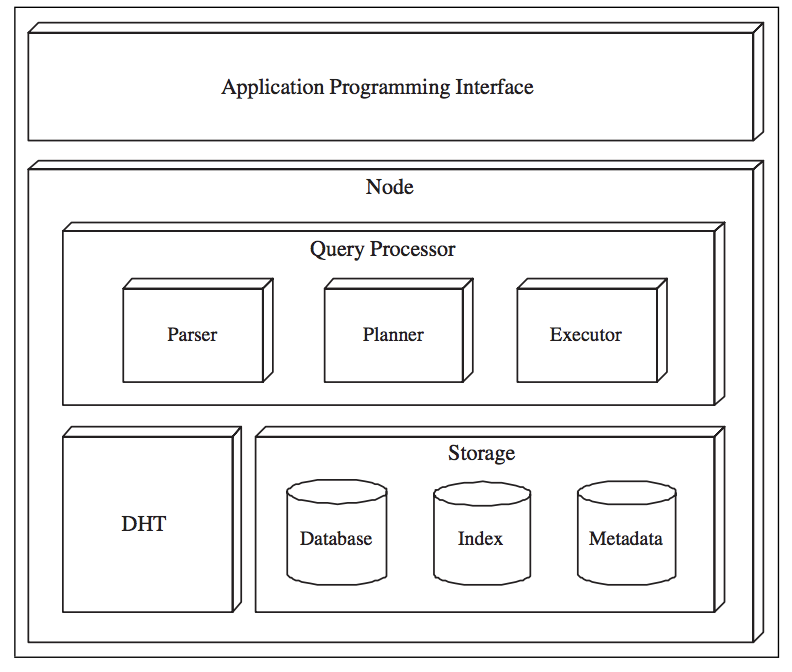
\includegraphics[width=\fscale{1}]{node_arch.png}
	\caption{A node}
	\label{fig:node_arch}
\end{figure}
The metadata in \figref{fig:node_arch} contains schema metadata to be exposed to the world. Nodes that wish to keep a table private should not have entries in metadata. Suppose there is a table called \textit{users} with four columns: \textit{username}, \textit{firstname}, \textit{lastname} and \textit{email}. The exported metadata entry might look like:
\begin{center}
	\begin{tabular}{| c | c |} 
		\hline
		Entity & Keywords \\ [0.5ex] 
		\hline
		users & user, people, customer, profile\\ 
		\hline
		name & name \\
		\hline
		firstname & fn, {f\_name}, {first\_name} \\
		\hline
		lastname & ln, {l\_name}, {last\_name} \\
		\hline
		email & id, contact \\ [1ex] 
		\hline
	\end{tabular}
\end{center}
When a query is posed to any node in the system, the node first tries to fulfill it with a local query before passing it along to its neighbors. Remember, nodes in the system host data with heterogeneous schemas. Similarity metrics that determine whether a query matches a heterogeneous schema are not discussed here.
\newline
\newline
\textbf{Dynamic clustering}:
Semantic proximity metrics are used to find nodes that are hosting semantically similar schemas. Overtime, these nodes are discovered and are clustered together for better query performance by reducing the number of network hops required.
\newline
\newline
\textbf{Data sovereignty}: 
Picolo supports two different schema types: \textit{application controlled} and \textit{user controlled}. Applications can use user controlled schemas to put users in absolute control of data and better comply with regulations like GDPR. For example, a decentralized twitter may  want users to have control over their tweets. Users can use any third party client or Picolo's official clients to interact with their tweets effectively rendering the decentralized twitter just another client albeit with better features.

When semantics don't allow to put user in control of data, application controlled schemas can be used. An example here would be a decentralized ticketing application where users should not be give fine grained control to selectively delete data about which tickets they bought.
\newline
\newline
\textbf{Access control}:
Applications and users may want to share data with other parties but may not need to impose access controls. There are a few ways of achieving this including building an API on top of the data or using proxy re-encryption techniques. We use a secret sharing scheme instead as it gels well with p2p nature of the system and does not introduce asymmetry like other solutions. Rules can be defined by a SQL like declarative language at any granularity desired including at the level of a single row and cell. An example row level granularity rule looks like:\newline \newline
\texttt{ SELECT  * \newline FROM users \newline WHERE email=foo@bar.com \newline NODE (SELECT nodeId FROM nodes WHERE domain=application)} \newline \newline
An example value level (only username is given access to) granularity rule looks like:\newline \newline
\texttt{ SELECT username \newline FROM users \newline WHERE email=foo@bar.com \newline NODE (SELECT nodeId FROM nodes)}

\section{Verifiable data structures and Mechanism design}
See how trillian works, audit proofs, transaction logs can be verified. Different ways data can be encrypted.  Fully encrypted onlhy provides key value semantics, while no encryption provides full SQL semantics. In addition indexes can be used to have 'value lookups' where data is partially encrypted. User control of data

Trillian implements a Merkle tree whose contents are served from a data storage layer, to allow scalability to extremely large trees. On top of this Merkle tree, Trillian provides two modes:

An append-only Log mode, analogous to the original Certificate Transparency logs. In this mode, the Merkle tree is effectively filled up from the left, giving a dense Merkle tree.
A Map mode that allows transparent storage of arbitrary key:value pairs. In this mode, the key's hash is used to designate a particular leaf of a deep Merkle tree, giving a sparse Merkle tree. (A Trillian Map is an unordered map; it does not allow enumeration of the Map's keys.)

This can be used to construct proofs.

Possible attacks on the system

How cryptonomics can be leveraged to prevent such attacks

How is the system constructed to make sure that desired outcome is achieved

\section{MX Protocol}
This section only specifies the message exchange protocol of the system. Nodes in the network need to speak the same language for efficient discovery and communication of data. Hence the following message exchange scheme is proposed. Note that the exact mapping between the following messages and underlying transport protocol is not discussed here and may change depending on the final transport protocol chosen (QUIC vs TCP)
\newline
\newline
\textbf{PUT}:  A PUT message contains the query to be run, an optional list of nodes to run the query against and an optional max number of hops (needed in case of an empty node list). This is used for creating or updating data in the system.
\newline
\newline
\textbf{GET}: A GET message contains the query to be run, max number of hops, the number of results to retrieve, the mode of retrieval (pull vs push) and a transaction identifier. Client sends this to a server to retrieve results that match the query. Parameters in GET can be varied depending on application needs - a streaming application may choose the push mode in which server pushes data to the client as it becomes available up until the specified number is met. Another latency sensitive application may choose to retrieve a small number of results in a batch instead in one pull.
\newline
\newline
\textbf{SEND}: Server responds to each GET message with one or more SEND messages with results. In pull mode, there is only one SEND message followed by an END message where as in push mode there are multiple SEND messages followed by an END message.
\newline
\newline
\textbf{END}: Server sends END message to indicate to the client that it has finished sending all results in response to a particular GET message.
\newline
\newline
\textbf{CLOSE}: A client can send a CLOSE message to the server to indicate that it no longer is interested in the remaining query results and close the transaction. It doesn't have to wait until all the results are retrieved.
\newline
\newline
\textbf{OK}: Server sends this message to a client as a positive acknowledgment to the client's message.
\newline
\newline
\textbf{ERROR}: Server sends this message to a client as a negatively acknowledge to the client's message.

\section{EIP and EEA}
We are drafting an EIP to give ethereum dapp developers a new choice for data storage. Not all data need to be replicated on every full node of ethereum as the need for strongest security maybe an overkill for most smart contracts. Such data can be stored on Picolo network at a contract defined replication factor. Picolo may also be used by ``stateless clients" as the network to query for data that is normally hosted by ``archival nodes" in the current implementation or in the upcoming sharded implementation.
\newline\newline
Picolo fits well in the EEA stack as the solution for off-chain storage of structured data. With capabilities like access logs and fine grained access control, enterprises can confidently share data with third parties without the need for expensive and cumbersome API management solutions.

\end{document}
